%-----------------------------------------------------------------------------
%\section{Design of \ours{}}
\begin{figure}[t]
\centering
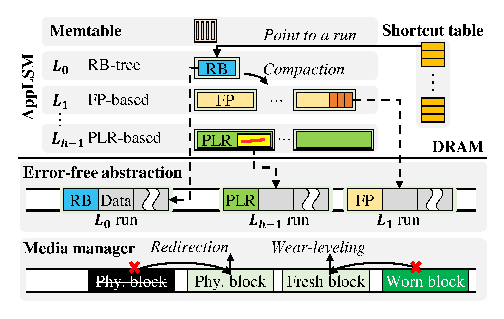
\includegraphics[width=0.37\textwidth]{figs/OSDI/koo/overall.eps}
\caption{Overall architecture of \ours{}}
\label{fig:overall}
\end{figure}

\section{Design and Implementation of \ours{}} 
\label{sec:new-design}
%This section describes the overall design of \ours{} and the techniques to
%reduce DRAM, flash writes, and reads.
\ours{} can be implemented in an OS kernel or in an SSD controller.
For typical SSDs that expose overwriteable logical blocks to the
host, \ours{} is implemented in an SSD controller as the form of firmware.
For latest ZNS SSDs~\cite{zns-ssd} and OCSSDs~\cite{ocssd} that expose
append-only media~\cite{dm-zoned}, \ours{} runs in OS's kernel
(\eg~\texttt{dm-zap}~\cite{dm-zap}), performing L2P indexing on the host
side.  For the sake of presentation, we assume that \ours{} is implemented in
an SSD controller.

In this section, we first explain the overall design of \ours{}, along with its
operations (\SEC{design:overall}). Then, we present how our approximate
algorithms work (\SEC{sec:design:fp}--\SEC{sec:design:plr-basic}).
Finally, we explain how \ours{} can be organized to provide reasonable WAFs
with minimal memory usages (\SEC{sec:combine}--\SEC{sec:design:tree}).


\subsection{Overall Organization} 
\label{design:overall}
%We explain key components that comprise \ours{} and associated data structures.
%Then, we present how \ours{} handles read and write requests.

%\textbf{System Components.}
\FIG{fig:overall} illustrates the overall organization of \ours{}
with its key components.
A \textit{media manager} is responsible for managing error-prone NAND
chips. It provides error-free NAND abstraction -- physical blocks 
and pages -- to upper-level components by internally performing bad-block 
management and  wear-leveling with a tiny redirection table. 

%NAND chips are shipped with bad blocks. As NAND blocks are erased repeatedly,
%moreover, they gradually wear out and become bad blocks.  Regardless of which
%index structure is used, SSD firmware should be able to manage error-prone NAND
%ㅈchips.  In \ours{}, a \textit{media manager} is responsible for managing NAND
%chips, providing error-free NAND abstraction (\ie~pages and blocks) to
%upper-level components.  For managing bad blocks and wear-leveling, it
%maintains a tiny redirection table that maps flash blocks (exposed to the upper
%layers) to NAND-device blocks.  Once a bad block is identified, the media
%manager excludes it by updating  the redirection table. It also internally
%performs wear-leveling for balanced block wearing. 
\begin{comment}
NAND chips are shipped with bad blocks. As NAND blocks are erased repeatedly,
moreover, they gradually wear out and become bad blocks.  Regardless of which
index structure is used, SSD firmware should be able to manage error-prone NAND
chips.  In \ours{}, a \textit{media manager} is responsible for managing NAND
chips, providing error-free NAND abstraction (\ie~pages and blocks) to
upper-level components.  For managing bad blocks and wear-leveling, it
maintains a tiny redirection table that maps flash blocks (exposed to the upper
layers) to NAND-device blocks.  Once a bad block is identified, the media
manager excludes it by updating  the redirection table. It also internally
performs wear-leveling for balanced block wearing. 
\end{comment}

Over the error-free NAND abstraction, 
\ours{} organizes its flash-resident data structures.
Individual runs are stored over physically continuous flash blocks (exposed by
the media manager). Each run is divided into metadata and data areas.
The metadata area keeps indices pointing to data in the data area
and is stored at the beginning of each run when
run's data is written to the flash.  
Flash-resident metadata is never used to locate data in the read path.  
It is only used for reconstructing its in-memory data
structures after system reboots.

\ours{} has four in-memory data structures: a \textit{memtable}, a
\textit{shortcut table}, and two types of \textit{approximate indices}.  
The memtable is equivalent to a write buffer. Its size is several MBs
(\eg~1MB$\sim$4MB) in size, and it is large enough to fully utilize write
throughput of NAND devices. The shortcut table is referenced to find a run that
has data to access.  It is an LBA-indexed flat table, each entry of which
points to a run where a logical block is stored.  \ours{} usually maintains 29
runs in the tree, so 5-bit per entry is enough to locate all possible runs.
For individual runs, \ours{} maintains approximate indices, 
in-memory copies of run's metadata. 
Two different algorithms, \textit{fingerprint} (FP)- and
\textit{PLR-based approximation}, are used to build approximate
indices. Each run chooses one that requires less memory.

%The shortcut table is more memory efficient than typical bloom filters.  When
%we build bloom filters using the same amount of memory, it suffers from an FPR
%of 0.091, but the shortcut table ensures an FPR of 0.0.  Be advised that the
%shortcut table is applicable only a key is an integer and the maximum number
%of items to store is determined when designing the system like \ours{}.

%When a write request comes, \ours{} buffers its data in a memtable that is
%equivalent to a write buffer in an SSD. Like conventional SSDs, the memtable
%is several MBs (\eg~1MB$\sim$4MB) in size, but is large enough to fully
%utilize write throughput of NAND devices.

\textbf{I/O Operations.}
We explain how \ours{} handles write requests.  Incoming logical blocks
are first buffered in the memtable.  Once it becomes full, \ours{} flushes out
pending data to $L_0$.  \ours{} manages $L_0$ as a log,
appending pending data to $L_0$ without sorting through compaction.  This
approach is useful to remove I/O overheads caused by frequent compaction
between the memtable and $L_0$~\cite{rocksdb,leveldb}.  For fast query over $L_0$, \ours{}
maintains a \textit{red-black (RB) tree}.  
The RB-tree is tiny as $L_0$ is small in size. 

Once $L_i$ is filled with data, \ours{} flushes out 
the data of all runs in $L_i$ to a new run in $L_{i+1}$
via compaction. 
%It is necessary to keep the tree sorted. 
%When writing data to a new run in $L_{i+1}$,
During compaction, 
\ours{} builds approximate indices and writes them to the metadata area 
of the new run.
Corresponding entries in the shortcut table must be updated 
accordingly to point to the new run.
In our design, compaction substitutes SSD's cleaning process
as the overall procedures of the two are almost the same; 
they read data from runs
(or victim blocks) and move them to a new run (or free space). 
The only difference is that \ours{} needs to sort data by LBA.  
\ours{} reduces compaction I/Os by excluding outdated data.
Existing LSM-trees move all data to a new run, including obsolete ones,
because of high tree lookup costs. On the other hand,
\ours{} can quickly identify whether a run has the latest version of 
data or not by referring to the shortcut table.

%Another difference is that, while
%SSD cleaning excludes outdated data (which were overwritten by new data),
%LSM-tree moves all the data in runs to a new run, including obsolete ones.
%This is because high lookup cost. To identify outdated data, it has to look up
%the tree. \ours{} can easily identify obsolete data by referring to the shortcut
%table, lowering compaction costs.


%Except that the compaction needs to sort data by keys, the overall procedures of
%LSM-tree's compaction and FTL's GC are identical; they read data from runs (or
%victim blocks), exclude invalid ones, and write them to free space. 
%\koo{However, for the lowest level $L_{h-1}$, the compaction of \ours{} performs differently
%from that of LSM-trees. In LSM-trees,
%there is no limit in the height of the tree.
%Thus, once the last level $L_{h-1}$ becomes full, they create a new last level $L_{h}$
%and move data to it. 기존 LSM-tree도 h가 시작 시에 정해져 있고, 마지막 레벨은 AppLSM과 비슷한 방식 아닌지 확인 필요.}
%On the other hand, \ours{} limits the tree height to $h-1$ as
%the creation of a new level requires additional DRAM to maintain indices.
%Instead, within the last level $L_{h-1}$,
%\ours{} repeats moving data in a victim run to a free run,
%filtering out invalid ones. 
%This is similar to what typical FTLs do for GC. 




\begin{comment}
\textbf{Data Structure.}
Once the memtable becomes full, \ours{} flushes out pending data to $L_0$. In
our design, $L_0$ has a single run. The run size is one of the configurable
parameters, and it usually ranges from 5MB to 5.4GB for a 1TB SSD. 
Since the 
run is larger than the memtable, \ours{} performs costly merge-sort operations
to maintain the sorted run in $L_0$, whenever the memtable is flushed out to
$L_0$.
%\cancel{\ours{} reads in data from $L_0$, merge-sorts them with those
%in the memtable, and finally writes them back to $L_0$.}  
To avoid costly
merge-sort operations, \ours{} manages $L_0$ as a log, appending data to
$L_0$ all the time. For fast query, \ours{} maintains exact indices for $L_0$
that hold <$x_i$, $y_i$> pairs sorted by $x_i$. $L_0$ is small in size, so DRAM
for the exact indices is tiny (\eg~10.8MB when the run size is
5.4GB). It is worth noting that some KV stores
employ the same approach to lessen flush overheads~\cite{rocksdb}.
\end{comment}

\begin{comment}
\textbf{Operations.}
%Besides $L_0$, the rest of levels $L_1$, ..., $L_{h-1}$ are managed in the same
The rest of levels $L_1$, ..., $L_{h-1}$ are managed in the same
manner as explained in \SEC{sec:back:lsm-tree}. Once $L_i$ is filled with data,
\ours{} flushes data from $L_i$ to $L_{i+1}$ through compaction to keep the
tree sorted.  The compaction is costly since it involves many I/Os,
increasing a write amplification factor (WAF) = 
($\frac{\text{data written to flash}}{\text{data written by host}}$).
\ours{}
reduces the number of I/Os for the compaction by adjusting the organization of a tree
(see \SEC{sec:design:tree}),
%\sout{and applying several optimization techniques (see \SEC{todo})}.
offering a sufficiently low WAF. However, the
resulting WAF is still higher than those of typical FTLs. This does not
diminish the value of \ours{} as reads have a higher impact on user-perceived
performance. Write throughput of SSDs can also be optimized in various
ways via write buffering~\cite{write-buffer}, 
write suspension/resume~\cite{suspension}, and
so on.
\end{comment}

%\ours{} handles a read query differently from typical LSM-trees.  
Given an LBA to query, \ours{} looks up the shortcut table
and finds a designated run that has a physical sector for the LBA.
Then, \ours{} searches for desired data in the run.
Each run is managed by different indexing strategies.
%\ours{} uses different indexing strategies for levels.  
If the run belongs to the $L_0$, 
\ours{} retrieves wanted data
by looking up the RB-tree.
%Through binary search, \ours{} can find an exact location of the given query.  
For the other levels that are managed by either FP- or PLR-based
indexing, \ours{} estimates the
location of the given LBA by following the approximate algorithm
and reads data from the suggested location.
If the location holds wrong data, 
\ours{} has to perform a local search
or moves to the next run to find the correct one.  
%A prediction error incurs extra I/Os.
%\JS{\sout{As such errors repeat, 
%the performance of \ours{} degrades significantly.}}

Prediction errors involve unnecessary I/Os.
Thus, a primary issue in designing \ours{} is how to
provide a low error rate while consuming as less memory as possible.
We discuss these issues in \SEC{sec:design:fp}--\SEC{sec:design:plr-basic}.
Besides accuracy and memory efficiency, 
we also present how we make index lookup faster,
which is another important design factor.
